%(BEGIN_QUESTION)
% Copyright 2007, Tony R. Kuphaldt, released under the Creative Commons Attribution License (v 1.0)
% This means you may do almost anything with this work of mine, so long as you give me proper credit

Ved observasjon av denne prosesstrenden ser vi variablene PV, SP og Output:

$$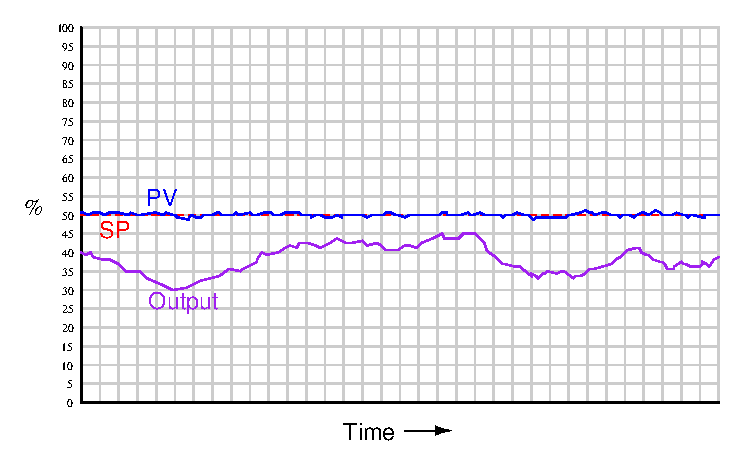
\includegraphics[width=15.5cm]{i01647x01.eps}$$

Setpunktet (SP) er den flate linjen ved 50\%. Prosessvariabelen (PV) er den svakt ujevne kurven som svinger rett over og under den flate setpunktlinjen. Utgangen er den svært urolige kurven under både PV- og SP-kurvene.

Operatøren for denne prosessen ringer deg, teknikeren, for å klage på reguleringskvaliteten i prosessen. Han hevder at regulatoren må tunes for å stabilisere Output-kurven slik at den ikke er så urolig. Basert på observasjonene av denne trenden, hva mener du skjer i prosessen? Trenger regulatoren tuning?

\vskip 10pt

Hva tror du vil skje hvis regulatoren settes i ``manuell'' modus? Hvordan vil det endre utseendet til prosesstrenden?

\vfil

\underbar{file i01647}
\eject
%(END_QUESTION)





%(BEGIN_ANSWER)

Dette er et vurdert spørsmål -- ingen svar eller hint er gitt!

%(END_ANSWER)





%(BEGIN_NOTES)

Det er ingenting galt med regulatorinnstillingen i denne prosessen. Kombinasjonen av stabil PV-trend og urolig utgangstrend indikerer at regulatoren gjør nøyaktig det den skal: holde prosessvariabelen ved setpunkt ved å justere manipulert variabel deretter.

Det som skjer i denne prosessen er at vi har varierende prosess{\it last} som tvinger regulatoren til å reagere ``urolig'' for å holde PV lik SP. Dette er ikke regulatorens feil, men et forhold i selve prosessen.

\vskip 10pt

Etter at regulatoren settes i ``manuell'' modus kan trenden se omtrent slik ut:

$$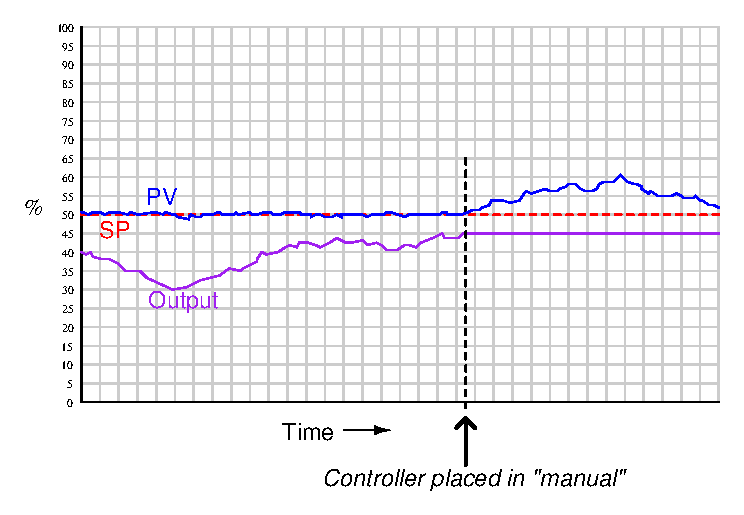
\includegraphics[width=15.5cm]{i01647x02.eps}$$

Når dette er sagt, må det påpekes at urolig utgangsvirkning fra regulatoren kan ha negative effekter på reguleringsventilen (dersom sluttregulerende element er en reguleringsventil), som for tidlig slitasje og lekkasje i pakkboks, samt høyt forbruk av trykkluft for pneumatiske aktuatorer (som er en løpende kostnad!). Den eneste måten å dempe dette på, bortsett fra å fjerne lastvariasjon i prosessen, er å tune regulatoren ned slik at den ikke reagerer så aggressivt på PV-endringer. Den negative konsekvensen er at PV ikke lenger vil holde seg like tett på setpunkt.

I praksis er situasjonen slik: så lenge variasjon i prosesslasten består, kan du ikke både ha robust regulering (lavt PV $-$ SP-avvik) {\it og} et stabilt utgangssignal. Du kan få det ene eller det andre (eller ingen av delene), men ikke begge.

I manuell modus blir Output-kurven en flat linje (fordi regulatoren holder utgangsverdien fast på det den var i øyeblikket ved overgang fra auto til manuell), og PV får ``vandre'' i takt med endringer i prosesslast. Her blir variasjoner i prosesslast tydelig synlige.

%INDEX% Control, PID tuning: manual mode as a diagnostic tool
%INDEX% Process troubleshooting: diagnosing problem via trend recording

%(END_NOTES)
